\documentclass[12pt,a4paper]{article}

\usepackage[utf8]{inputenc}
\usepackage[ngerman]{babel}
\usepackage[T1]{fontenc}
\usepackage{amsmath}
\usepackage{amsfonts}
\usepackage{amssymb}
\usepackage{graphicx}
\usepackage[left=2cm,right=2cm,top=2cm,bottom=2cm]{geometry}
\usepackage{multicol}
\usepackage{booktabs}
\usepackage[hidelinks]{hyperref}
\usepackage{tikz}
\usepackage{pgfplots}
\usepackage{blindtext}
\usepackage{array}
\usepackage{multirow}
\usepackage{bigdelim}
\usepackage{colortbl}
\usepackage{fancyhdr} 
\usepackage{tabularx}
\usepackage{pgfplots}
\usepackage{xcolor}
\usepackage{color}
\usetikzlibrary{decorations.text}
\usetikzlibrary{tikzmark}
\pagestyle{fancy} 
	\fancyhf{} 
	\fancyhead[L]{
\includegraphics[scale=0.05]{Bilder/dhbw.png}} 
	\fancyhead[C]{\slshape WLAN} 
	\fancyhead[R]{\slshape LaTeX Version}
	\fancyfoot[C]{\thepage}

\usepackage{helvet}
\renewcommand{\familydefault}{\sfdefault}

\newcolumntype{Z}{>{\centering\let\newline\\\arraybackslash\hspace{0pt}}X}
\author{\slshape Robin Rausch, Florian Maslowski, Ozan Akzebe}
\title{WLAN}
\date{\slshape \today}

\begin{document}
\maketitle
\tableofcontents
\newpage

\section{Zuständige Organisation und Normen}
IEEE legt verschiedenste Normen in der Computer Technik fest. Darunter auch alle Normen und Standards zum WLAN.\\
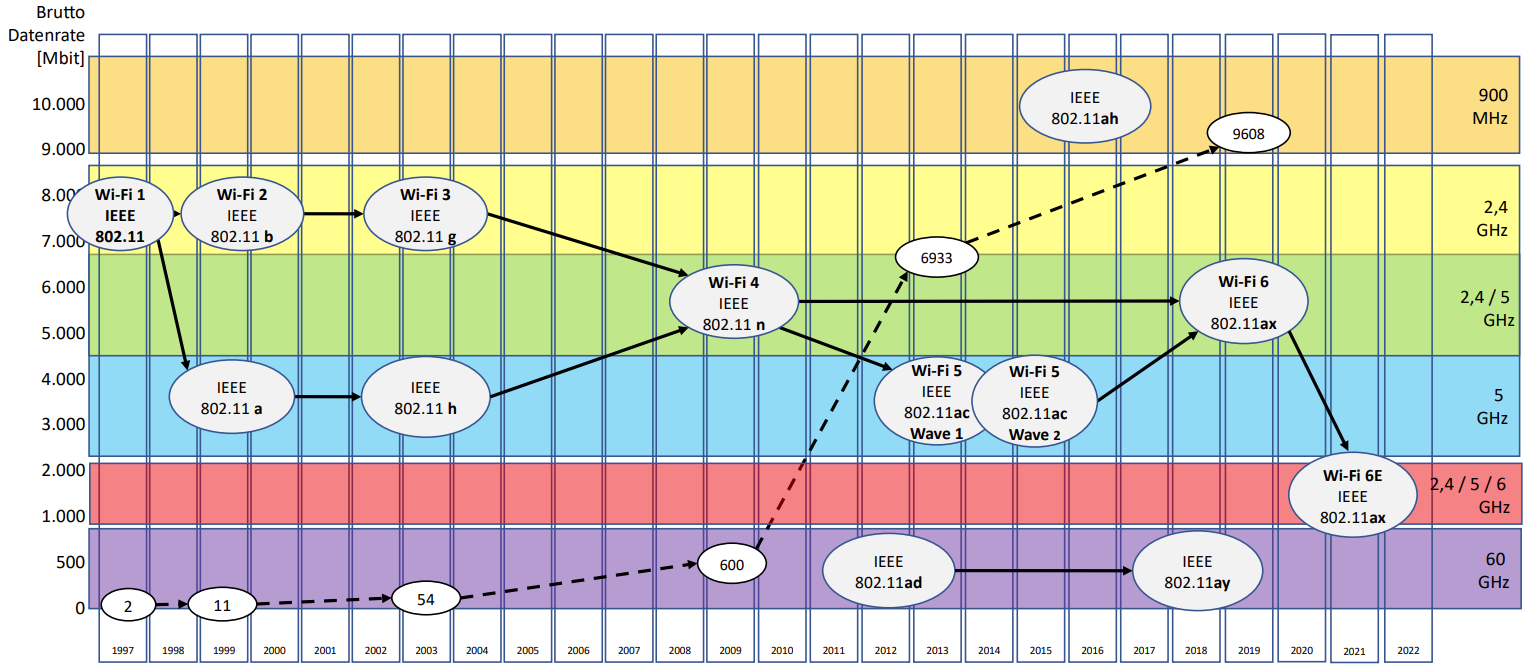
\includegraphics[width=\textwidth]{Bilder/wlan_standards_uebersicht.PNG}

\section{Funknetz}
	Base station-> Base station controller (BSC): verbindet Base stations-> Mobile switching center (MSC): verbindet BSC mit Festnetz (PSTN) und Internet-> externes Netzwerk.\\
	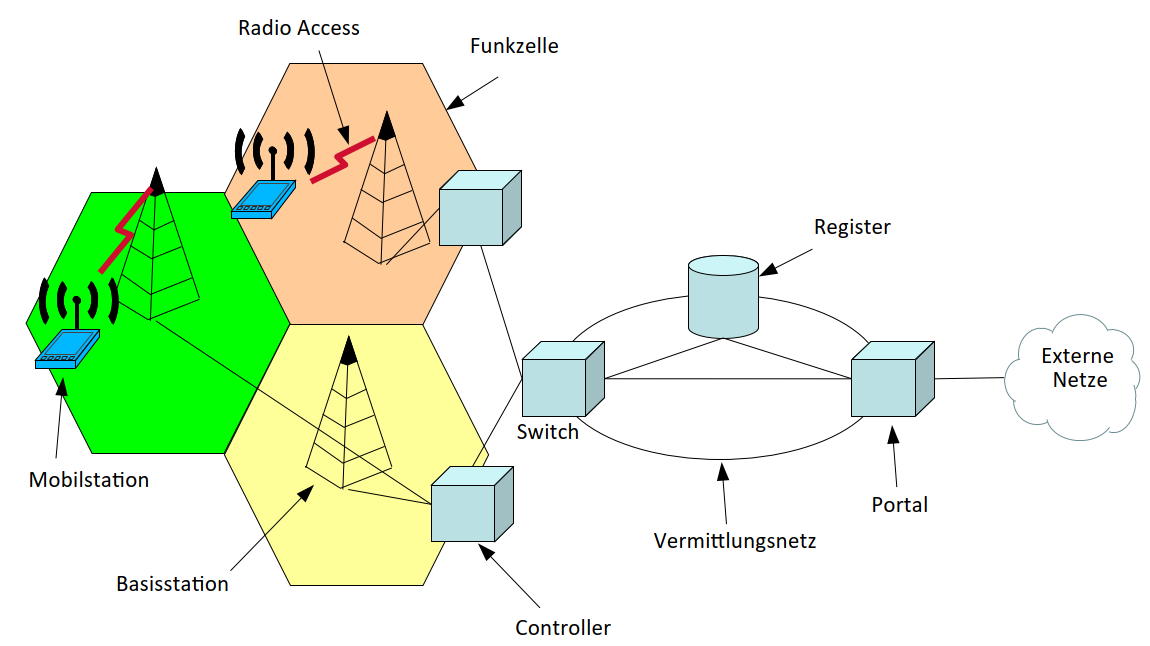
\includegraphics[width=\textwidth]{Bilder/Funknetz.png}

	\subsection*{Handover vs. Roaming}
		\textbf{Handover} ist Übergabe von Accesspoint zu Accesspoint im selben Subnetz (Layer 2).\\
		\textbf{Roaming} ist Übergabe von Accesspoint zu Accesspoint in anderes Subnetz (Layer 3). \\
		Die zwei Subnetze laufen unter verschiedenen Switches.

	\subsection*{Wiederverwendungsabstand}
		Basestations nebeneinander kommunizieren auf verschiedenen Frequenzbändern, um an Übergängen keine Störungen zu verursachen.\\
		Das selbe Frequenzband bekommen nur Stationen, welche mindestens eine Station zwischen sich haben.
	
\section{OFDM}
	Orthogonal Frequency-Division Multiplexing ist eine Methode zur digitalen Signalmodulation, bei dem ein einzelner Datenstrom auf mehrere separate Schmalbandkanäle mit unterschiedlichen Frequenzen aufgeteilt wird, um Interferenzen und Übersprechen zu reduzieren.
	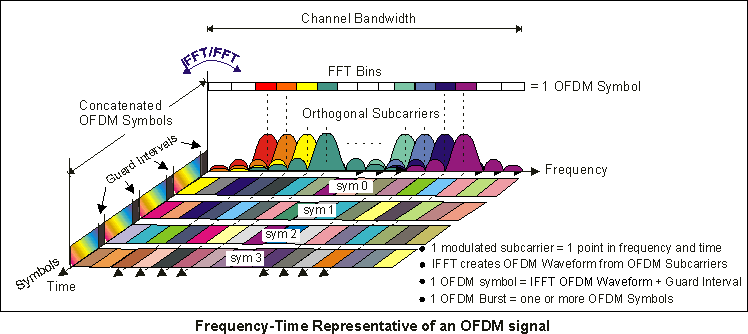
\includegraphics[width=\textwidth]{Bilder/ofdm.png}
	Lösungsansätze von OFDM sind BPSK, QPSK oder n-QAM(Bsp.: 16-QAM, 32-QAM, usw.).\\
	Ziel von OFDM ist möglichst viel Breitbandgewinn:\\
	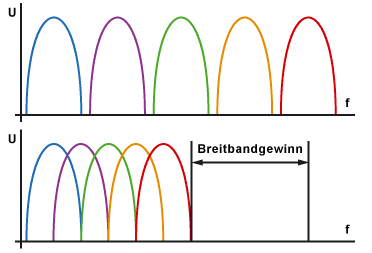
\includegraphics[width=0.5\textwidth]{Bilder/ofdm_breitbandgewinn.PNG}
	
	\subsection{Viterbi-Algorithmus}
		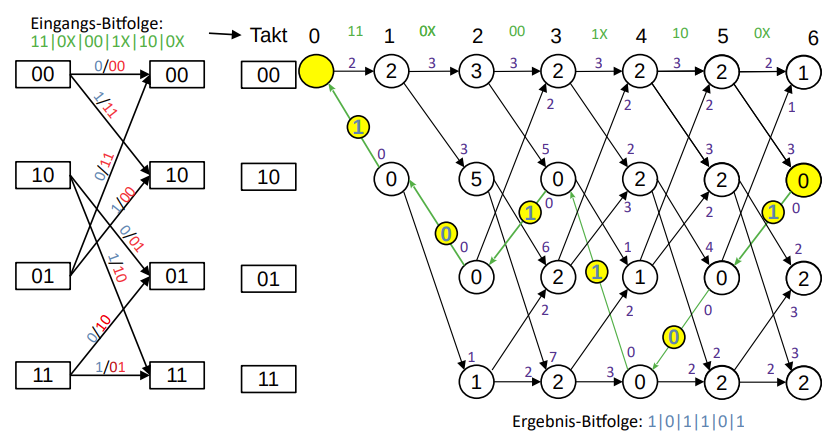
\includegraphics[width=\textwidth]{Bilder/viterbi.PNG}

	\subsection{OFDM-Faltungskodierer}
		OFDM (Orthogonal Frequency Division Multiplexing) ist eine Modulationstechnik, die häufig in drahtlosen Kommunikationssystemen wie WLAN, LTE und 5G verwendet wird. OFDM teilt das verfügbare Frequenzspektrum in eine große Anzahl schmaler Unterkanäle auf, die als Träger oder Subträger bezeichnet werden. Jeder Subträger verwendet eine niedrigere Symbolrate als der gesamte Signalstrom, was zu einer erhöhten Robustheit gegenüber Kanalstörungen führt.\\
		Ein Faltungskodierer ist ein Fehlerkorrekturverfahren, das verwendet wird, um die Zuverlässigkeit der Datenübertragung zu verbessern. Er fügt dem ursprünglichen Datenstrom Redundanz hinzu, indem er zusätzliche Bits generiert, die Informationen über die ursprünglichen Daten enthalten. Diese zusätzlichen Bits ermöglichen es dem Empfänger, Fehler zu erkennen und zu korrigieren.\\
		Ein OFDM-Faltungskodierer kombiniert die Vorteile von OFDM und Faltungscodes, um die Datenübertragungseffizienz und die Fehlertoleranz in drahtlosen Kommunikationssystemen zu verbessern. Der Faltungskodierer wird vor der Modulationsschicht in den OFDM-Block eingefügt.\\
		Der OFDM-Faltungskodierer besteht aus zwei Hauptkomponenten: dem Faltungscodierer und dem Interleaver.\\
		Faltungscodierer: Der Faltungscodierer nimmt den Datenstrom als Eingabe und erzeugt einen codierten Datenstrom mit zusätzlicher Redundanz. Er verwendet eine spezielle Art von Codierungsalgorithmus, der als Faltungscodierung bezeichnet wird. Dieser Algorithmus basiert auf einer Verschieberegisterstruktur und kombiniert die Eingabebits durch XOR-Operationen. Der Ausgabestrom des Faltungscodierers enthält sowohl die ursprünglichen Datenbits als auch die codierten Redundanzbits.\\
		Interleaver: Der Interleaver nimmt den codierten Datenstrom vom Faltungscodierer und ändert die Reihenfolge der Bits, um die Auswirkungen von Burstfehlern zu verringern. Durch die Umordnung der Bits werden die codierten Bits auf verschiedene Subträger verteilt, was dazu beiträgt, die Auswirkungen von Kanalstörungen gleichmäßig zu verteilen und zu verringern.\\
		Der OFDM-Faltungskodierer ermöglicht eine effiziente und zuverlässige Datenübertragung in drahtlosen Kommunikationssystemen. Er verbessert die Fehlererkennung und -korrektur und trägt zur Verbesserung der Bitfehlerrate und der Gesamtleistung des OFDM-Systems bei.\\
		Hierzu wird des Viberti-Algorithmus verwendet.

	\subsection{Datenrate berechnen}
		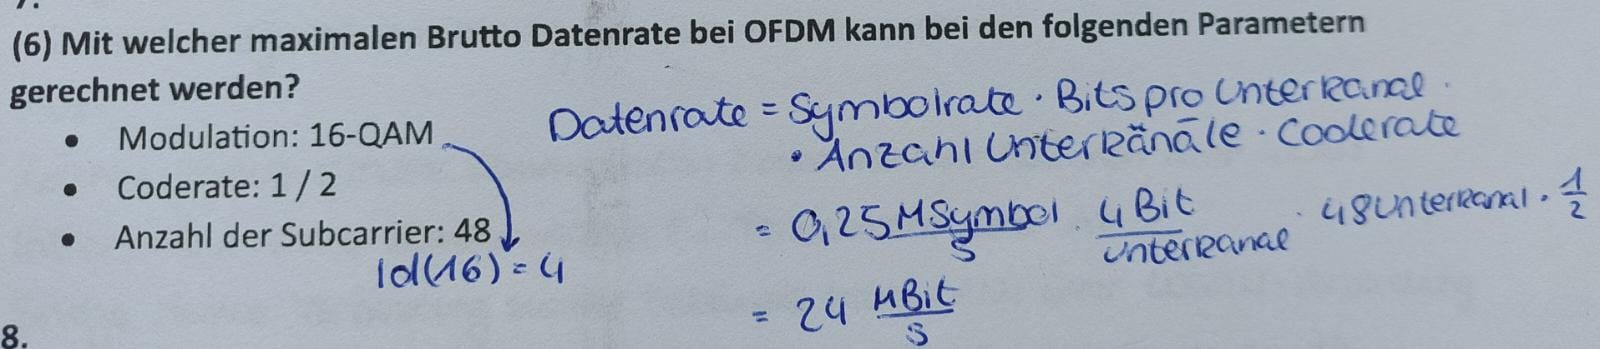
\includegraphics[width=\textwidth]{Bilder/datenrate_berechnen.jpg}

\section{OFDMA}
	OFDMA steht für ''Orthogonal Frequency Division Multiple Access'' und ist eine Zugriffsmethode, die in drahtlosen Kommunikationssystemen, insbesondere in Wi-Fi-Netzwerken der nächsten Generation (z. B. Wi-Fi 6 und Wi-Fi 6E), eingesetzt wird.\\
	OFDMA basiert auf der Technologie der Orthogonalen Frequenzmultiplexierung (OFDM), bei der das Frequenzspektrum in schmale Unterkanäle unterteilt wird. Bei OFDMA wird jeder Unterkanal weiter in kleinere Frequenzbänder aufgeteilt, die als Ressourcenblöcke bezeichnet werden. Diese Ressourcenblöcke können dann verschiedenen Benutzern oder Geräten zugeordnet werden, um gleichzeitig und effizient Daten zu übertragen.\\
	Der Hauptvorteil von OFDMA besteht darin, dass es die gleichzeitige Übertragung mehrerer Datenströme ermöglicht, indem es das Frequenzspektrum effizient aufteilt und Ressourcenblöcke dynamisch an verschiedene Benutzer oder Geräte zuweist. Dadurch wird die Kapazität des drahtlosen Netzwerks erhöht, die Latenz reduziert und die Gesamtleistung verbessert. OFDMA wird häufig in Umgebungen eingesetzt, in denen viele gleichzeitige Verbindungen und eine hohe Datendichte vorhanden sind, wie zum Beispiel in dicht besiedelten städtischen Gebieten.\\
	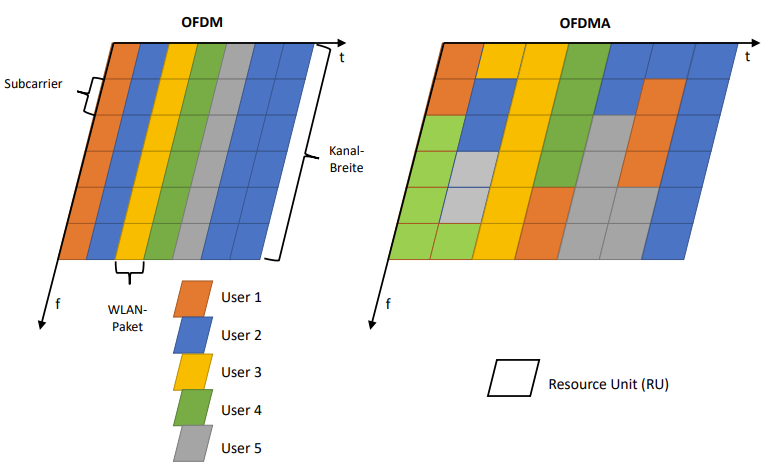
\includegraphics[width=\textwidth]{Bilder/ofdma.PNG}

\section{Modi}
	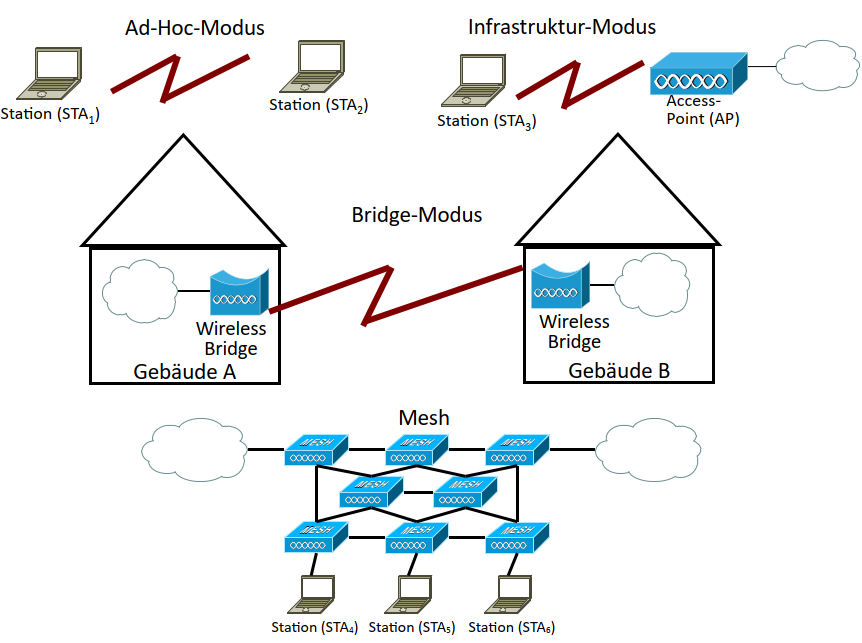
\includegraphics[width=0.7\textwidth]{Bilder/Funkmodi.png}

	\begin{description}
		\item[BSS:] Basic Service Set: Ist WLAN nach IEEE 802.11
		\item[STA:] Station 
		\item[IBSS:] Independent Basic Service Set: Ist Netzwerk mit mehreren WLAN-Clients ohne Anschluss zu externem Netz. Topologie wird auch Ad-Hoc bezeichnet.
		\item[BSS Infrastruktur mode:] BSS mit Anschluss zu externem Netzwerk (über Accesspoint) 
		\item[Bridge:] Netze drahtlos verbinden
		\item[Mesh:] 
	\end{description}

\section{WLAN-Standards}
	Nach Übertragungskapazität sortiert:
	\begin{description}
		\item[802.11 ah:] 900 MHz
		\item[802.11:] 2.4 GHz
		\item[802.11 b:] 2.4 GHz
		\item[802.11 a/h/g:] 5 GHz/5 GHz/2.4 GHz
		\item[802.11 n:] 2.4 GHz \& 5 GHz
		\item[802.11 ac:] 5 GHz
		\item[802.11 ax:] 2.4 GHz \& 5 GHz \& 6 GHz
		\item[802.11 ad:] 60 GHz
		\item[802.11 ay:] 60 GHz
	\end{description}

\section{Sicherheit}
	\textbf{Radius Server:} zentraler Authentifizierungsserver, an den sich Services für die Authentifizierung von Clients in einem physischen oder virtuellen Netzwerk (VPN) wenden.\\
	\textbf{File Server:}  Computer, der für das Speichern und Verwalten von Datendateien eingesetzt wird, damit andere Computer im selben Netzwerk auf die Dateien zugreifen können.

\section{Mobile IP}
Netzprotokoll-Standard, um Benutzern von mobilen Geräten wie Notebooks den Wechsel von einem Rechnernetz in ein anderes zu ermöglichen und dabei gleichzeitig eine feste IP-Adresse zu behalten.

\section{Multiplex-Verfahren}
	\begin{description}
		\item[Time Division Multiplexing] Basestations senden/empfangen mit verschiedenen Clients zu verschiedenen Zeiten.
		\item[Frequency Division Multiplexing] Basestations senden/empfangen auf anderen Frequenzen.
		\item[Space Division Multiplexing] Basestations senden/empfangen an anderen Orten.
		\item[Codec Division Multiplexing] Basestations senden/empfangen mit anderen Codecs.
		\item[Orthogonal Frequency Division Multiplexing(OFDM)] Sonderform von FDM. Durch Orthogonalität Übersprechen der Träger reduzieren.
		\item[Orthogonal Frequency Division Multiple Access] Anstatt dass ein User alles bekommt (OFDM), wird der Träger in Unterträger/ Resource Units(RU) aufgeteilt und auf max. 9 User verteilt.  
	\end{description}

\section{Physical (PHY)-Layer}
	\begin{description}
		\item[Signalspreizung] Schwache Signale empfangen.
	\end{description}
	\subsection{Frequency Hopping Spread Spectrum (FHSS)}
	Data-Link besteht aus MPDU.\\
	PHY besteht aus Präampel(144/72 Bits) und Physical Layer Convergence Protocol (PLCP)-Header.
	Präampel besteht aus Sync und Start Frame Delimiter(SFD).\\
	Präampel besteht aus 80 Bit 0101...\\
	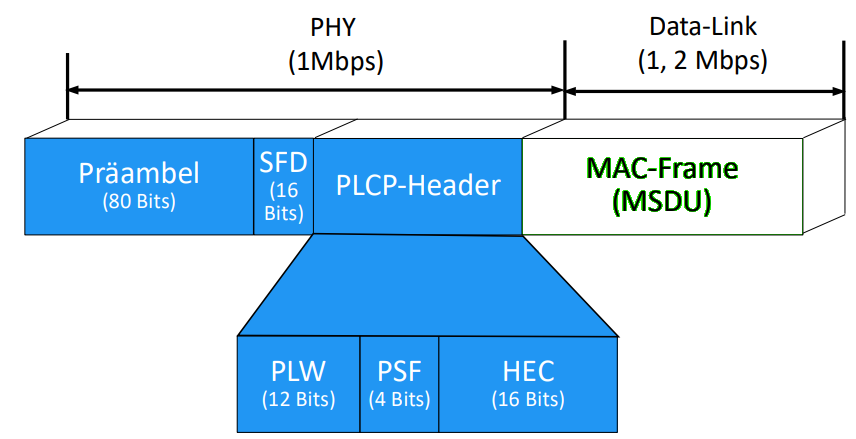
\includegraphics[scale=0.6]{Bilder/FHSSFrame-removedBg.png}

\section{Hamming Code}
	Code zur Fehlerkorrektur mit Paritätsbits.\\
	Unfunktionell bei mehr als einem Fehlerbit.\\
	Alle $2^n \; (n \in \mathbb{N}_0)$ Bits sind Paritätsbits => Skaliert gut für große Blöcke.
	Die Positionsnummern der 1er-Bits werden ohne Übertrag aufsummiert und das Ergebnis wird in die Paritätsbits geschrieben.
	\begin{center}
		\begin{tabular}{ |c|c|c|c|c|c|c|c| } 
		 \hline
		 \textbf{Werte} & 1 & 0 & 1 &  & 0 &  & \\ 
		 \hline
		 \textbf{Positionsnummer} & \color{green}7 & 6 & \color{blue}5 & 4 & 3 & 2 & 1\\ 
		 \hline
		\end{tabular}
	\end{center}
	Paritätsbits berechnen:
	\begin{center}
		\begin{tabular}{ c c c c c } 
		  & \color{green}1 & \color{green}1 & \color{green}1 & \\ 
		  + & \color{blue}1 & \color{blue}0 & \color{blue}1 &  \\ 
		 \hline
		 = & \color{red}0 & \color{red}1 & \color{red}0 &  \\ 
		\end{tabular}
	\end{center}
	Wird zu:
	\begin{center}
		\begin{tabular}{ |c|c|c|c|c|c|c|c| } 
		 \hline
		 \textbf{Werte} & 1 & 0 & 1 & \color{red}0 & 0 & \color{red}1 & \color{red}0\\ 
		 \hline
		 \textbf{Positionsnummer} & 7 & 6 & 5 & 4 & 3 & 2 & 1\\ 
		 \hline
		\end{tabular}
	\end{center}
	
	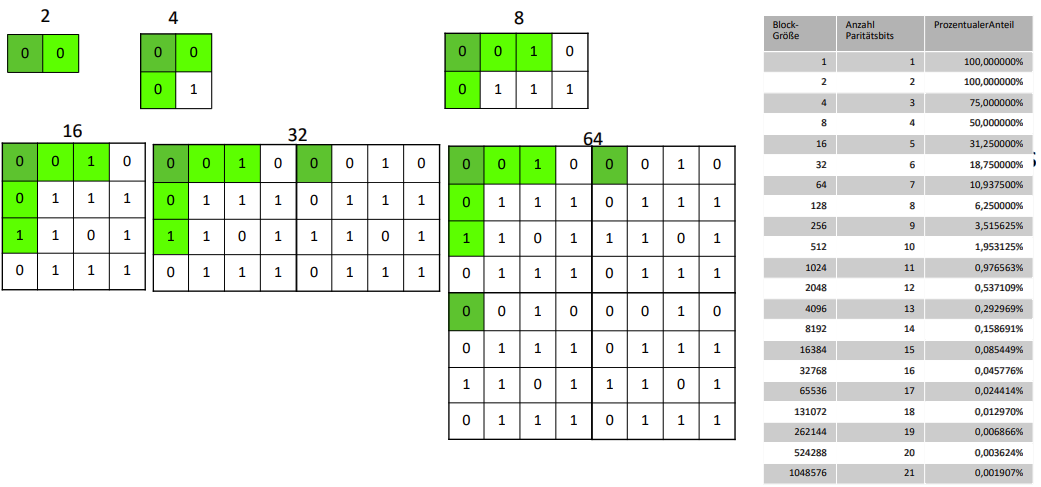
\includegraphics[width=\textwidth]{Bilder/hamming_code-removedBg.png}

\section{Medien Datenübertragung}
	\subsection{MAC-Ebene \& Frames}
		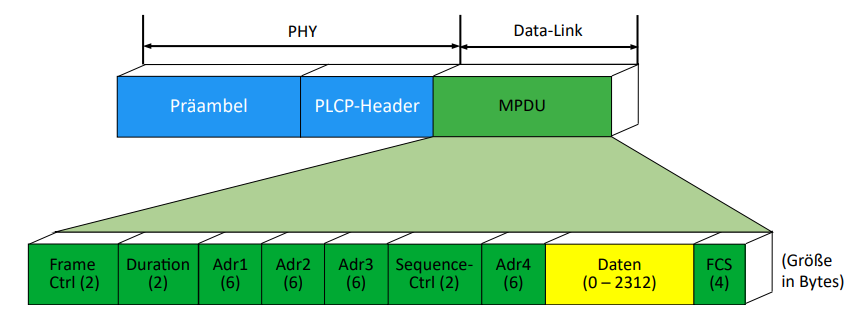
\includegraphics[scale=0.7]{Bilder/MAC Ebenene.png}\\
		\subsubsection{Kontrollfeld aufbau:}
		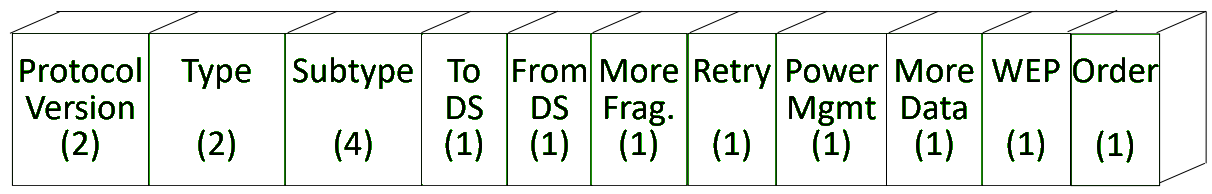
\includegraphics[scale=0.4]{Bilder/Control field structure-removedBg.png}
		\begin{description}
			\item[PLCP:] Physical Layer Convergence Protocol. 
			\item[MPDU:] MAC (Media Access Control) Protocol Data Unit 
			\item[FCS:] Prüfsumme
		\end{description}

	\subsection{WLAN Aufgaben in der OSI Schicht 2 - MAC-Ebene}
		\begin{itemize}
			\item Adressierung
			\item Zugriffsverfahren CSMA/CA
			\item Bilden von Prüfsummen
			\item Quittieren(ACK)
			\item Fragmentierung und Reassemblierung
			\item Verschlüsselung
		\end{itemize}

	\subsection{Medium Zugriffe}
		\subsection{Hidden Station Problem}
			Wenn Sta1 und Sta2 sich nicht sehen und Accesspoint B von beiden gesehen wird, fangen Sta1 und Sta2 an zu senden. Dies kann zu Kollisionen führen.\\
			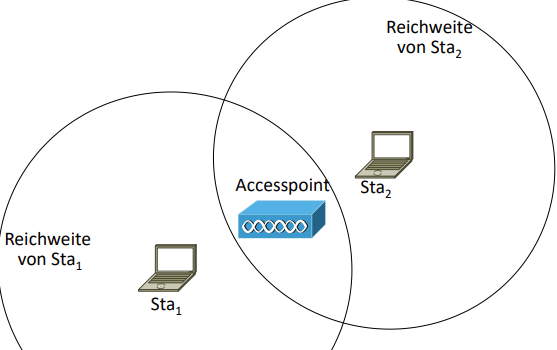
\includegraphics[width=0.5\textwidth]{Bilder/hidden_station_problem.PNG}

		\subsection{Exposed Station Problem}
			Wenn in unserem vorliegenden Szenario die Sta1 an Sta4 sendet und nun Sta2 an irgendeine andere Station senden möchte, die nicht im Sendebereich von Sta1 liegt. Dadurch wartet Sta2 unnötig auf das Ende des Datenaustauschs.\\
			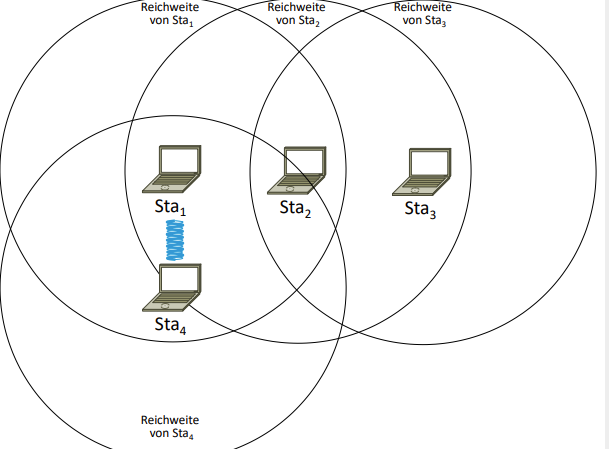
\includegraphics[width=0.5\textwidth]{Bilder/exposed_station_problem.PNG}\\
			\vspace{2cm}\\
			\textbf{\underline{Um diese Probleme zu vermeiden gibt es:}}

		\subsubsection*{Distributed Coordination Function(DCF)}
			Zugriffsverfahren über alle Teilnehmer verteilt realisieren.\\
			Kollisionsauflösung durch beispielsweise CSMA/CA

		\subsubsection*{Carrier Sense Multiple Access/Collision Avoidance(CSMA/CA)}

		\subsubsection*{Request To Send/Clear To Send(RTS/CTS)}
			Optionaler Zusatz für CSMA/CA, um hidden-station-Problem zu vermindern. Steht für Request-to-Send/Clear-to-Send. RTS frägt Zielstation ob sie frei ist. Wenn das der Fall ist antwortet diese mit CTS und teilt somit auch allen anderen umliegenden Stationen mit, dass diese nun belegt ist.\\\\
			\textbf{NAV - Network Allocation Vector}\\
			Der NAV ist eine Zeitvariable, die dazu dient, die Übertragung von Datenpaketen zwischen verschiedenen Teilnehmern eines WLANs zu koordinieren. Im Wesentlichen wird der NAV von einem drahtlosen Gerät verwendet, um andere Geräte im Netzwerk darüber zu informieren, dass es beabsichtigt, den Kanal für eine bestimmte Zeitdauer zu nutzen. Der NAV wird verwendet, um Kollisionen zu verhindern, wenn mehrere Geräte gleichzeitig versuchen, Daten zu senden. Wenn ein Gerät Daten senden möchte, überprüft es zuerst den NAV-Wert des Kanals. Ist der NAV-Wert größer als Null, bedeutet dies, dass ein anderes Gerät den Kanal bereits für die Übertragung reserviert hat. In diesem Fall wartet das sendende Gerät, bis der NAV-Wert auf Null gesunken ist, was darauf hinweist, dass der Kanal frei ist.\\
			Der NAV wird durch sogenannte Request to Send (RTS) und Clear to Send (CTS) Frames aktualisiert. Ein Gerät sendet ein RTS-Feld, um anderen Geräten im Netzwerk mitzuteilen, dass es den Kanal für eine bestimmte Zeitdauer nutzen wird. Wenn kein Konflikt besteht, antwortet das Empfängergerät mit einem CTS-Feld, das den NAV-Wert entsprechend aktualisiert.\\
			Der NAV löst somit das Hidden Station Problem.
		
		\subsubsection*{Point Coordination Function(PCF)}
			Optionaler Zusatz für CSMA/CA, bei welchem der Accesspoint die Medienzugriffe zentral steuert.

		\subsubsection*{IFS}
		Inter Frame Spaces sind Zeitspannen, die in drahtlosen Netzwerken verwendet werden, um den Zugriff auf den drahtlosen Kanal zu regeln. IFS bestimmen die Wartezeit, die zwischen der Übertragung von Rahmenpaketen verschiedener Sender im Medium verstreichen muss.\\
		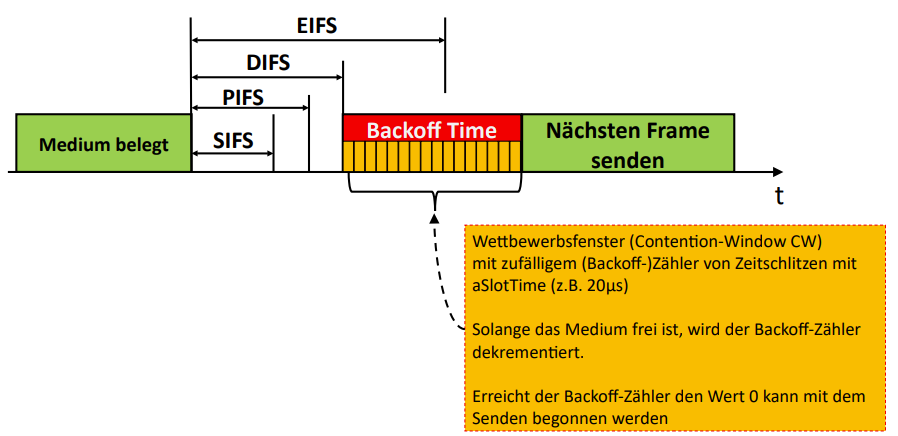
\includegraphics[width=\textwidth]{Bilder/ifs.PNG}
		\textbf{SIFS} Short Inter Frame Space\\
		\textbf{PIFS} PCF Inter Frame Space\\
		\textbf{DIFS} Distributed Inter Frame Space\\
		\textbf{EIFS} Extended Inter Frame Space \\

	\subsection{Zeitsynchronisation/Fragmentierung}
		Zeitsynchronisation im WLAN bezieht sich auf die Synchronisierung der Geräte im Netzwerk, um den Zugriff auf den Funkkanal zu koordinieren. Dadurch können sie effizient senden und empfangen, um Kollisionen zu vermeiden.\\
		Fragmentierung ist die Aufteilung großer Datenmengen in kleinere Fragmente für eine zuverlässigere Übertragung. Es ermöglicht Fehlererkennung, Robustheit gegenüber Störungen und eine effizientere Nutzung des Funkkanals.\\
		Insgesamt helfen Zeitsynchronisation und Fragmentierung dabei, die Leistung und Zuverlässigkeit von WLAN-Netzwerken zu verbessern.

	\subsection{ManagementFrames}
		Management Frames sind eine Art von Rahmenpaketen in drahtlosen Netzwerken, die zur Verwaltung und Steuerung des Netzwerkbetriebs verwendet werden. Diese Rahmenpakete dienen der Kommunikation zwischen den drahtlosen Stationen (Geräten) und dem Access Point (AP) und enthalten Informationen, die für die Netzwerkverwaltung, Authentifizierung, Verbindungsaufbau und -abbau, sowie für das Monitoring und die Fehlerbehebung relevant sind.\\
		Hier sind einige wichtige Arten von Management Frames:
		\begin{description}
			\item[Beacon Frames:] Beacon Frames werden vom Access Point periodisch ausgesendet und enthalten grundlegende Informationen über das drahtlose Netzwerk, wie den Netzwerknamen (SSID), die unterstützten Datenraten, die Verschlüsselungsmethode und weitere Parameter. 
			Diese Frames ermöglichen es drahtlosen Stationen, das Netzwerk zu erkennen und eine Verbindung herzustellen.
			\item[Probe Request/Response Frames:] Probe Request Frames werden von drahtlosen Stationen gesendet, um nach verfügbaren Netzwerken in der Umgebung zu suchen. Der Access Point antwortet mit Probe Response Frames, die detaillierte Informationen über das Netzwerk enthalten. Dadurch können die Stationen die besten verfügbaren Netzwerke auswählen.
			\item[Authentication Frames:] Authentication Frames werden während des Authentifizierungsprozesses zwischen einer drahtlosen Station und dem Access Point ausgetauscht. Sie dienen dazu, die Identität der Station zu überprüfen und sicherzustellen, dass sie Zugriff auf das Netzwerk erhalten kann.
		\end{description}

	\subsection{BSS-Coloring}
	BSS Coloring kennzeichnet nebenliegende WLAN Netzwerke mit unterschiedlichen Farbcodierungen um die Unterscheidung zwischen diesen zu erleichtern. Diese Farbcodierungen wird über Management Frames übergeben.

\section{Übertragung}		
	\subsection{Beamforming}
		Frequenzmanagement für Netze wie WLAN. Nur mit mindestens 2 Antennen(MIMO) möglich. Funktioniert durch ausfündigmachen der Clients und anpassen der verschiedenen Antennensendestärken. Wenn Wellen interferieren, ist das Signal stärker -> Antennen so einstellen, dass der Client in interferierenden Zonen ist.\\
		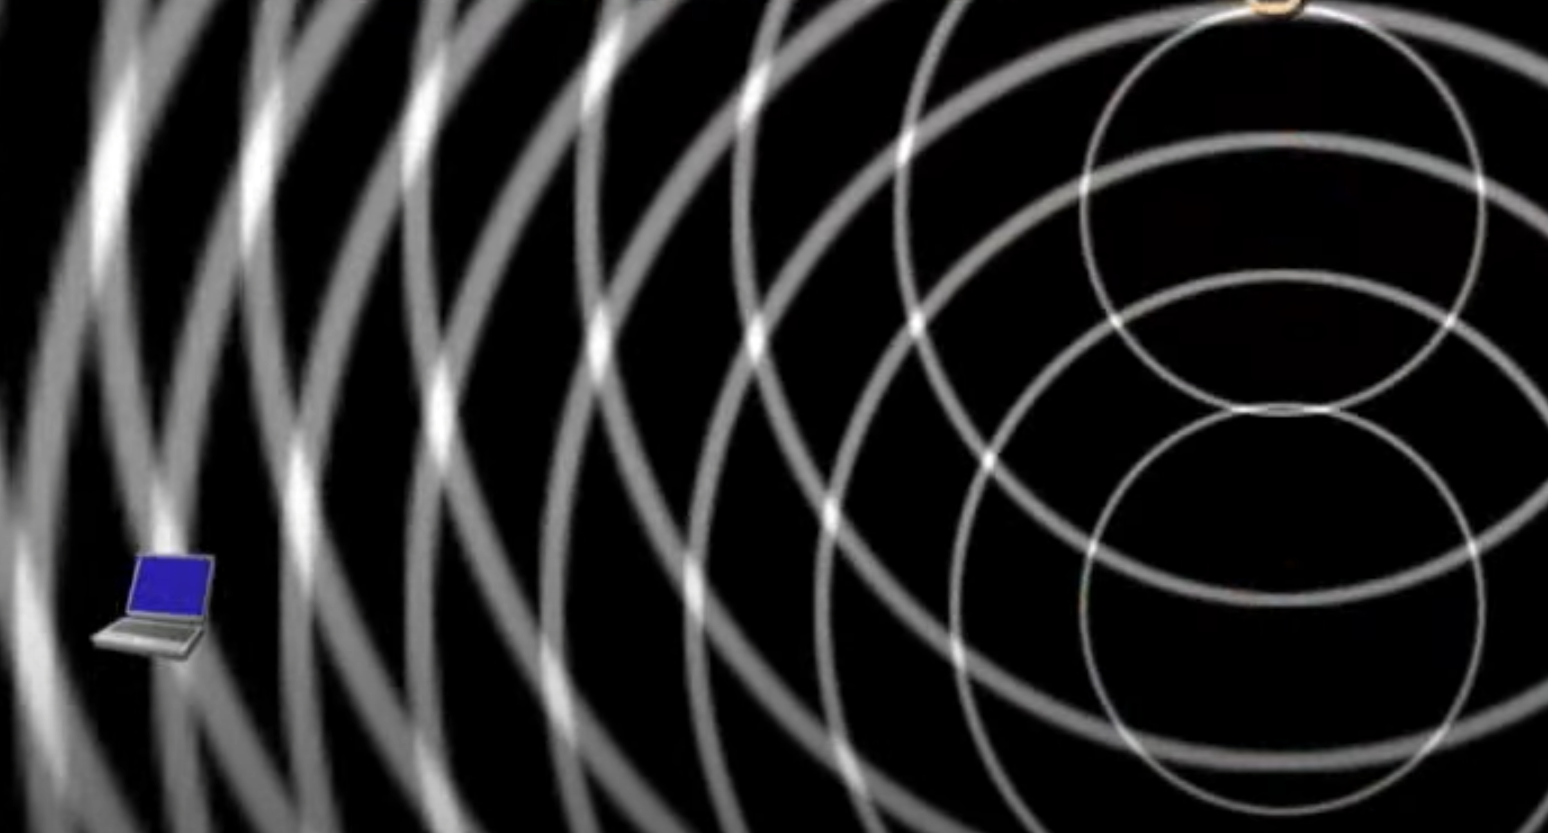
\includegraphics[width=0.5\textwidth]{Bilder/Beamforming.png}\\

	\subsection{Blockacknowledgement}
		ACK steht für ''Acknowledgment'' und ist eine Bestätigungsnachricht, die den erfolgreichen Empfang von Daten bestätigt. 
		''Block ACK'' ist eine erweiterte Version von ''ACK'', die die Bestätigung mehrerer Datenframes in einem einzigen Paket ermöglicht und die Effizienz der Datenübertragung verbessert (Verbesserung der MAC Effizienz). \\
		Sender: Nach mehreren Datenpacketen (Datenblock), Acknowlegde Request senden. \\
		Empfänger: Block Acknowlegdement senden.\\
		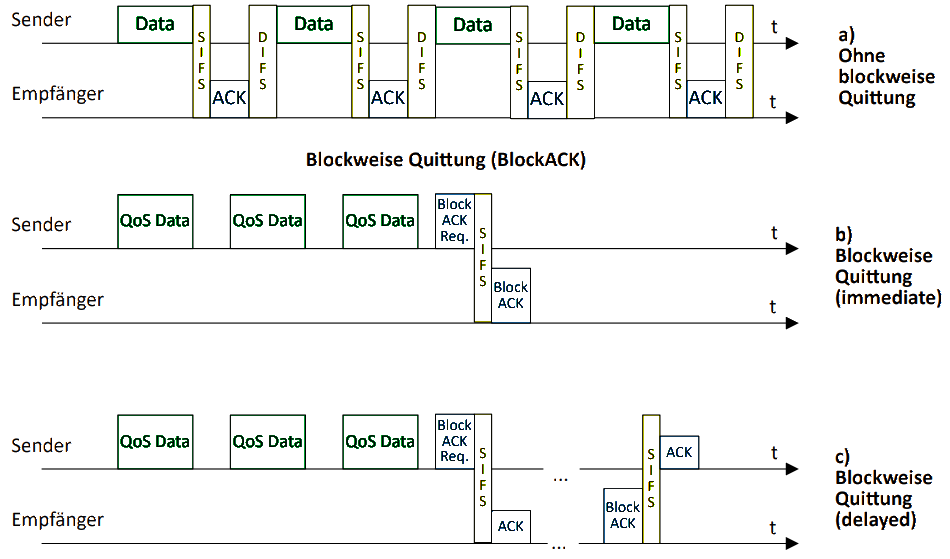
\includegraphics[width=\textwidth]{Bilder/Blockacknowlegdement-removedBg.png}\\
		(SIFS = Short Interframe Space: erforderliche Zeit bei drahtloser Übertragung, welche es abzuwarten gilt)

	\subsection{Power over Ethernet}
		Strom über das achtadrige RJ45 Kabel übertragen.\\
		-> Stromkabel kann gespart werden und es spart etwas Strom.\\
		- Es kann zur Überhitzung kommen
	
	\subsection{Verbindungsvorgang}
		\begin{enumerate}
			\item Scanning
			\item Authentifizierung von Station über Accesspoint mithilfe eines Authentification Servers
			\item Assoziation
		\end{enumerate}

		\subsubsection{Scanning}
		\textbf{Active}: Client sendet Prüfanfrage wartet auf Prüf Antwort vom AP.\\
		\textbf{Passive}: Client wartet/hört auf Beaconframes vom AP.\\

		\subsubsection{Authentifizierung}
			Die Authentifizierung kann durch zwei Möglichkeiten erfolgen:\\\\
			\begin{minipage}[t]{.45\textwidth}
				\subsubsection*{Open-System-Authentication}
				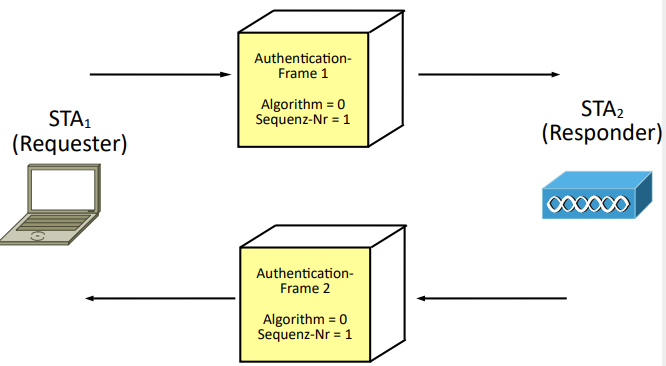
\includegraphics[width=\textwidth]{Bilder/os_auth.PNG}
			\end{minipage}
			\hspace{0.1\textwidth}
			\begin{minipage}[t]{.45\textwidth}
				\subsubsection*{Shared-Key-Authentication}
				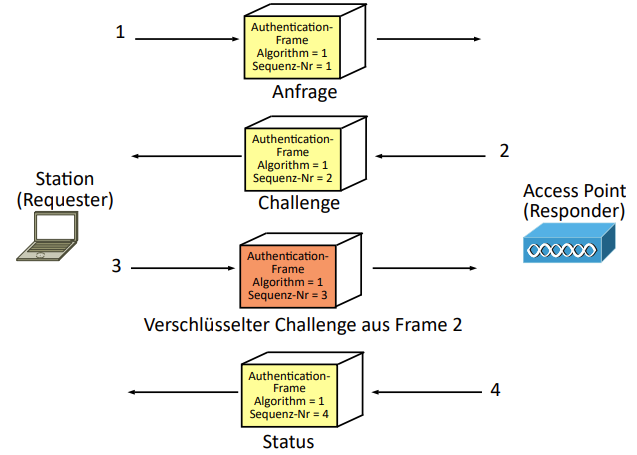
\includegraphics[width=\textwidth]{Bilder/sk_auth.PNG}
			\end{minipage}

		\subsubsection{Assoziierung}
			Bei der Assoziierung werden grundlegende Informationen zur Verbindung ausgetauscht. Die Assoziierung dienst der eindeutigen Identifikation.
	
	\subsection{QoS - Quality of Service}
	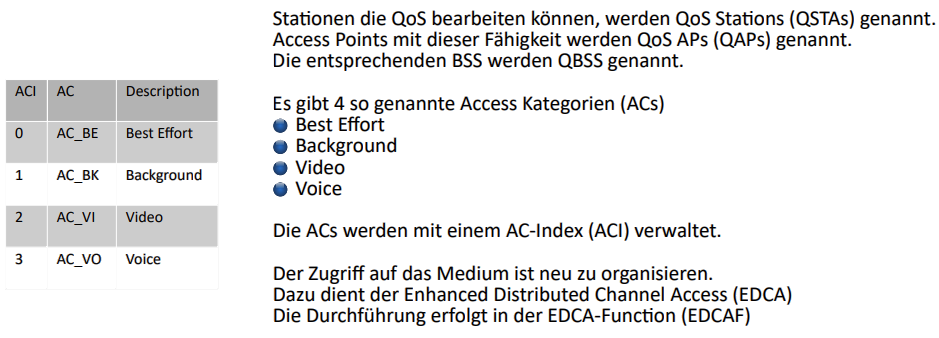
\includegraphics[width=\textwidth]{Bilder/QoS-removedBg.png}

\section{Antennen}
	\textbf{Masthöhe} muss mit Erdkrümmung berechnet werden.\\
	\textbf{Physikalisch:} Magnetfelder an Antennenstab aufbauen. 
	Durch Umpolen, und durch den Memoryeffekt des Magnetfeldes, wird das Magnetfeld abgeschnitten und vom neuen, umgekehrten Feld abgestoßen. \\
	\textbf{Halbwellendipol:}\\
	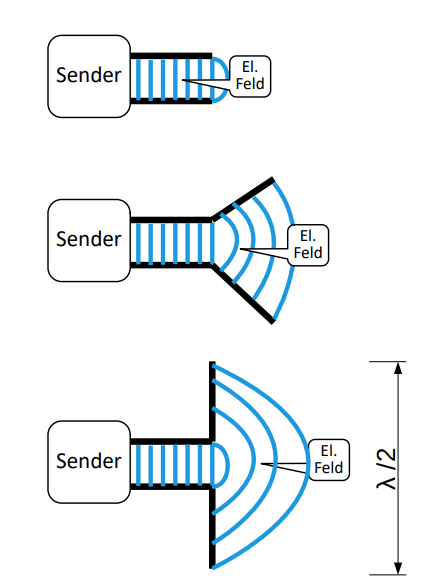
\includegraphics[scale=0.6]{Bilder/Halbwellendipol.png}\\
	
	\subsection{SISO vs. MIMO}
		Single Input Single Output benötigt eine Antenne pro Station.\\
		Multiple Input Multiple Output benötigt mindestens zwei Antennen pro Station, um die Datenkapazität und Robustheit in drahtlosen Kommunikationssystemen zu erhöhen (Sende- und Empfangsantenne).

		\subsubsection{MU-MIMO}
		MU-MIMO steht für Multi-User Multiple-Input Multiple-Output und ermöglicht die gleichzeitige Übertragung von Datenströmen an mehrere Empfänger in Wi-Fi-Netzwerken. Es verbessert die Effizienz und Kapazität des Netzwerks, besonders in Umgebungen mit vielen gleichzeitig aktiven Benutzern.

	\subsection{Antennen Arten}
	\begin{description}
		\item[Dipol] 
		\item[Geschlossene Dipol]
		\item[Patch] Erzeugt Halbkugelförmige Felder -> Gut für gleichmäßige Ausbreitung(Innenräume)
		\item[Isotrop] Punktförmig, verlustfrei, gleichmäßige Ausbreitung
		\item[Richtantennen] Gitterförmig, Feinfühliger, verschiedene Stäbe für verschiedene Zwecke (Reflektor, Dipol Antenne, Direktoren)
	\end{description}
	\textbf{Faktoren für Reichweite:}\\
	Sendeleistung, Reguläre Dämpfung durch Hindernisse, Störsignale, Verluste in Steckern / Anlagen / Kabeln \\\\
	\textbf{Freiraumdämpfung} ist die Abschwächung des Signals über Entfernungen. Welle 
	\textbf{Wichtige Begriffe:}
	\begin{description}
		\item[dB] dezibel
		\item[dBi] Antennen-/Leistungsgewinn im Bezug auf Isotropantenne
		\item[dBm] Logarithmische Wertangabe für Signalstärke (z.B. im WLAN)\\
		$dBm = 10 \log _{10} (\frac{P_{Antenne}}{P_{Bezugsantenne}})$
		\item[dBa] Leistungspegel
	\end{description}

	\subsection{Arten von Widerstand bei Funkwellen}
	\begin{itemize}
		\item Absorption
		\item Reflexion
		\item Transmission(geht durch)
		\item Beugung
	\end{itemize}

	\subsubsection{Antennengewinn berechnen}
		$G = 10 \cdot log_{10}(\frac{P}{P0})$\\\\
		Dabei steht P für die tatsächliche Ausgangsleistung der Antenne in Watt und P0 für die Ausgangsleistung eines isotropen Strahlers mit derselben Eingangsleistung. Der Antennengewinn wird in Dezibel angegeben, daher wird die logarithmische Funktion log10 verwendet.

	\subsubsection{EIRP - Equivalent Isotropic Radiated Power}
		EIRP (dBm) = Tx Power (dBm) - cable loss (dB) + Antennengewinn(dBi)

\section{World Mode}
	Der ''World Mode'' ermöglicht drahtlosen Geräten den Betrieb in verschiedenen Ländern mit unterschiedlichen Funkstandards. Die Länderkennung ist eine Information in den Geräten, die angibt, in welchem Land sie verwendet werden. Sie gewährleistet, dass die Geräte den regulatorischen Anforderungen des jeweiligen Landes entsprechen, einschließlich Frequenzbändern und Sendeleistungsbegrenzungen. Zusammen ermöglichen World Mode und Länderkennung den reibungslosen Betrieb drahtloser Geräte unter Einhaltung der gesetzlichen Vorgaben.\\
	Deutschland hat die Länderkennung 44 45.

\section{Wireshark}
	''Sniffer'', um Daten im Netzwerk mitzulesen.\\
	Platzierung ist auf einer Station im Netzwerk.\\
	Ein Filter beim Aufzeichnen hilft, um nicht unzählig viel Datenverkehr aufzuzeichnen und die Nadel im Heuhaufen zu suchen.
	
\section{Sicherheit}
	\textbf{Folgende Aspekte sollten bei einer Datenübertragung erfüllt werden:}
	\begin{itemize}
		\setlength\itemsep{0cm}
		\item Authentizität
		\item Datenintegrität
		\item Vetraulichkeit
		\item Verfügbarkeit
		\item Verbindlichkeit
		\item Anonymisierung
	\end{itemize}
	\textbf{Erreicht werden soll dies durch:}
	\begin{itemize}
		\setlength\itemsep{0cm}
		\item Authentifizierung bei der Anmeldung
		\item Verschlüsselung bei der Datenübertragung 
		\item eindeutige Sequenznummern und Prüfsummen zum Schutz der Datenintegrität
	\end{itemize}
	
	\subsection{WEP-Verschlüsselung}
		Wired Equivalent Privacy ist das ehemalige Standard-Verschlüsselungsprotokoll für WLAN. 
		Es sollte sowohl den Zugang zum Netz regeln als auch die Vertraulichkeit und Integrität der Daten sicherstellen. 
		Aufgrund verschiedener Schwachstellen gilt das Verfahren grundlegend als unsicher.\\
		WEP hat ein symmetisches Verschlüsselungsverfahren, jedoch kein Schlüssel-Management. 
		Es kann ''relativ'' einfach geknackt werden und authentifiziert keinen Benutzer, sondern einen Adapter.\\
		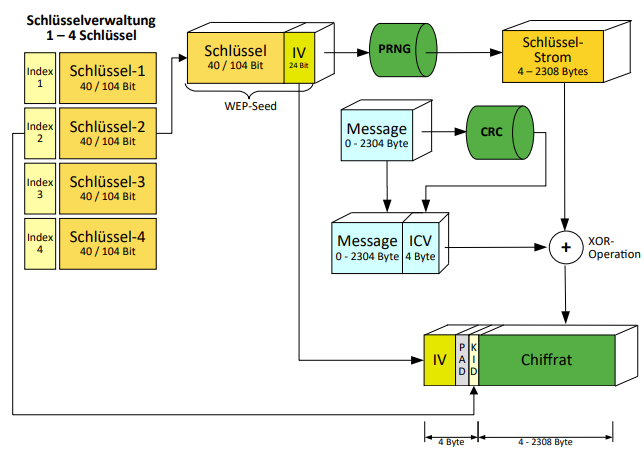
\includegraphics[width=0.8\textwidth]{Bilder/wep.PNG}

	\subsection{Wi-Fi Protected Access (WPA)}
		Die Sicherheitsarchitektur wurde aufgrund Sicherheitslücken in Wired Equivalent Priovacy (WEP) von 802.11 entwickelt.\\
		Folgende neue Features:
		\begin{enumerate}
			\item Packete müssen verschlüsselt und authentifiziert sein
			\item Ein Schlüssel nur für ein Paket benutzen
			\item Pakete haben unveränderbare Seqenznummer
			\item Kommunikationspartner müssen sich gegenseitig authentifizieren
		\end{enumerate}

	\subsection{WPA 2}
		WPA (Wi-Fi Protected Access) und WPA2 sind Sicherheitsprotokolle, die in WLAN-Netzwerken zum Schutz der drahtlosen Kommunikation eingesetzt werden. Sie wurden entwickelt, um die Schwachstellen des älteren WEP (Wired Equivalent Privacy) zu beheben und eine sicherere Datenübertragung zu gewährleisten. WPA verwendet den Verschlüsselungsalgorithmus TKIP (Temporal Key Integrity Protocol), während WPA2 den verbesserten Verschlüsselungsalgorithmus CCMP (Counter Mode with Cipher Block Chaining Message Authentication Code Protocol) verwendet.

		\subsubsection{TKIP (Temporal Key Integrity Protocol)}
			TKIP ist ein Verschlüsselungsalgorithmus, der in WPA verwendet wird. Es wurde entwickelt, um die Sicherheit von WEP zu verbessern, indem es dynamische Schlüssel generiert und einen stärkeren Verschlüsselungsmechanismus bietet. TKIP verwendet einen 128-Bit-Schlüssel und stellt zusätzliche Sicherheitsfunktionen wie eine Integritätsprüfung für die übertragenen Daten bereit.

		\subsubsection{CCMP (Counter Mode with Cipher Block Chaining Message Authentication Code Protocol)}
			CCMP ist ein Verschlüsselungsalgorithmus, der in WPA2 verwendet wird. Es bietet eine verbesserte Sicherheit im Vergleich zu TKIP. CCMP verwendet den AES (Advanced Encryption Standard) mit einer Schlüssellänge von 128 Bit für die Datenverschlüsselung und eine Authentifizierungsmethode namens MIC (Message Integrity Check) zur Überprüfung der Integrität der übertragenen Daten. Wird innerhalb von 60 Sekunden eine MIC Fehler erkannt, wird von einer Attacke ausgegangen und die Verbindung wird abgebrochen. Dies kann von beiden Seiten (Stationen oder AP) ausgehen (abhängig von Senderichtung).\\
			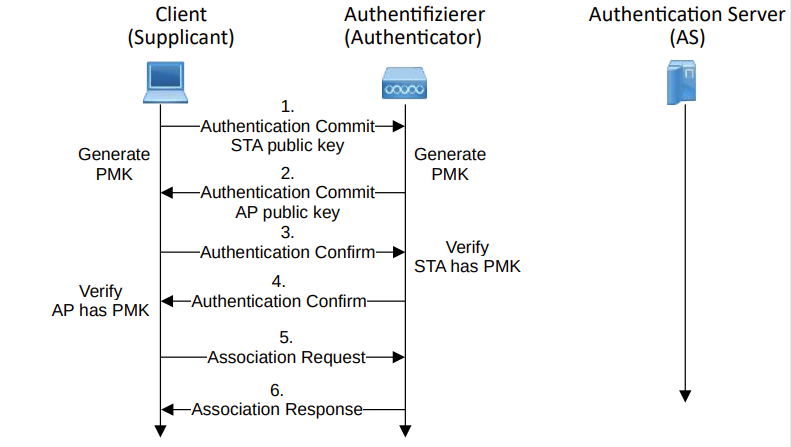
\includegraphics[width=\textwidth]{Bilder/wpa3.PNG}

	\subsection{WPA 3}
		WPA3 ist die neueste Version des Wi-Fi Protected Access-Protokolls. Es wurde entwickelt, um die Sicherheit und den Datenschutz in WLAN-Netzwerken weiter zu verbessern. WPA3 bietet neue Sicherheitsfunktionen wie individuelle Datenverschlüsselung für jedes Gerät im Netzwerk, Schutz vor Brute-Force-Angriffen und verbesserte Sicherheit bei öffentlichen WLAN-Netzwerken. Es ist wichtig zu beachten, dass WPA3 nicht rückwärtskompatibel zu älteren Geräten ist, die möglicherweise nur WPA/WPA2 unterstützen.

	\subsection{Kryptografie}
		\subsubsection{Symetrische Verschlüsselung}
			Symmetrische Verschlüsselung ist eine Form der Verschlüsselung, bei der derselbe Schlüssel sowohl für die Ver- als auch für die Entschlüsselung der Daten verwendet wird. Das bedeutet, dass Sender und Empfänger denselben geheimen Schlüssel teilen, der für die Verschlüsselung der Daten am Sender und die anschließende Entschlüsselung am Empfänger verwendet wird.

		\subsubsection{Asymetrische Verschlüsselung}
			Asymmetrische Verschlüsselung, auch Public-Key-Verschlüsselung genannt, ist ein Verfahren, bei dem zwei unterschiedliche Schlüssel für die Ver- und Entschlüsselung verwendet werden. Diese Schlüssel werden als öffentlicher Schlüssel und privater Schlüssel bezeichnet.\\
			Der öffentliche Schlüssel wird zum Verschlüsseln der Daten verwendet und kann frei verteilt werden. Jeder, der Zugriff auf den öffentlichen Schlüssel hat, kann damit Daten verschlüsseln, jedoch nicht entschlüsseln.\\
			Der private Schlüssel wird geheim gehalten und nur dem Empfänger bekannt gemacht. Er wird zum Entschlüsseln der mit dem öffentlichen Schlüssel verschlüsselten Daten verwendet.\\
			Der Vorteil der asymmetrischen Verschlüsselung besteht darin, dass es nicht erforderlich ist, den privaten Schlüssel zu teilen oder zu übertragen. Dadurch wird das Problem der sicheren Schlüsselverteilung gelöst. Die Vertraulichkeit der Kommunikation wird durch den privaten Schlüssel gewährleistet, der nur dem Empfänger bekannt ist.

	\subsection{Andere}
		Versteckte Nachrichten senden (Steganografie)\\
		Nachrichten geheim senden.\\
		Nicht im WLAN relevant

\section{Planung eines WLAN Netzwerkes}
	Bei der Planung	eines WLAN Netzes, sollte man sich vorher ausreichend über die Anforderungen informieren. 
	Gegebenheiten vor Ort, können ebenfalls zu Problemen führen und müssen bei der Planung beachtet werden. 
	Die Ausleuchtung einer Fläche kann folgende Stati annehmen:
	\begin{itemize}
		\item Abdeckungsorientiert
		\item Kapazitätsorientiert 
		\item Verfügbarkeitsorientiert
	\end{itemize}
	Bestehende Netze können beispielsweise mithilfe einer Heatmap analysiert werden. 

\end{document}